\documentclass[conference]{IEEEtran}
\IEEEoverridecommandlockouts
% The preceding line is only needed to identify funding in the first footnote. If that is unneeded, please comment it out.
\usepackage{cite}
\usepackage{amsmath,amssymb,amsfonts}
\usepackage{algorithmic}
\usepackage{graphicx}
\usepackage{textcomp}
\usepackage{xcolor}
\def\BibTeX{{\rm B\kern-.05em{\sc i\kern-.025em b}\kern-.08em
    T\kern-.1667em\lower.7ex\hbox{E}\kern-.125emX}}
\begin{document}

\title{From Macro Goals to Adaptive Skills:\\ Dialogue Policy Learning under Intent Drift}

\author{\IEEEauthorblockN{1\textsuperscript{st} Given Name Surname}
\IEEEauthorblockA{\textit{dept. name of organization (of Aff.)} \\
\textit{name of organization (of Aff.)}\\
City, Country \\
email address or ORCID}
\and
\IEEEauthorblockN{2\textsuperscript{nd} Given Name Surname}
\IEEEauthorblockA{\textit{dept. name of organization (of Aff.)} \\
\textit{name of organization (of Aff.)}\\
City, Country \\
email address or ORCID}
\and
\IEEEauthorblockN{3\textsuperscript{rd} Given Name Surname}
\IEEEauthorblockA{\textit{dept. name of organization (of Aff.)} \\
\textit{name of organization (of Aff.)}\\
City, Country \\
email address or ORCID}
\and
\IEEEauthorblockN{4\textsuperscript{th} Given Name Surname}
\IEEEauthorblockA{\textit{dept. name of organization (of Aff.)} \\
\textit{name of organization (of Aff.)}\\
City, Country \\
email address or ORCID}
\and
\IEEEauthorblockN{5\textsuperscript{th} Given Name Surname}
\IEEEauthorblockA{\textit{dept. name of organization (of Aff.)} \\
\textit{name of organization (of Aff.)}\\
City, Country \\
email address or ORCID}
\and
\IEEEauthorblockN{6\textsuperscript{th} Given Name Surname}
\IEEEauthorblockA{\textit{dept. name of organization (of Aff.)} \\
\textit{name of organization (of Aff.)}\\
City, Country \\
email address or ORCID}
}

\maketitle

\begin{abstract}
Traditional goal-oriented dialog agents require inefficient retraining when new objectives arise. While recent multi-objective methods parameterize goals, they rely on rigid numerical preference vectors. This misaligns with real-world settings, where macro-goals are expressed in natural language, requiring strategic flexibility and non-negotiable constraints. Furthermore, existing policies ignore intent drift, maintaining static behavior rather than adapting to evolving dialog contexts. To address these gaps, we propose \textbf{ALMOND}, a novel hierarchical framework for learning dialog policies. A \textit{low-level policy} executes communication skills via a regret-based mechanism, prioritizing unmastered skills to bootstrap complex behaviors robustly. Concurrently, a \textit{high-level policy} adaptively selects short-term skills by monitoring intent shifts, leveraging strategic hints distilled during training to satisfy the overarching linguistic goal. Extensive experiments show ALMOND significantly outperforms baselines. Our framework achieves superior linguistic goal completion, minimizes constraint violations, drastically reduces adaptation latency, and establishes a new state-of-the-art for short-term success rates.
\end{abstract}

\begin{IEEEkeywords}
goal-oriented dialogue, multi-objective reinforcement learning, intent drift,
dialogue policy planning, negotiation, conversational recommendation
\end{IEEEkeywords}
\section{Introduction}

Goal-oriented dialogue agents are increasingly expected to act on behalf of
users, not simply to generate fluent responses. In buyer-side negotiation, for
example, a useful agent must pursue a favorable price while keeping the seller
engaged, reaching an agreement within a limited number of turns, and respecting
the buyer's budget. Target-driven recommendation involves a similar balancing
act: the agent should guide the user toward a desired item without degrading
satisfaction or conversational efficiency. These objectives are not independent.
An aggressive bargaining move may improve price utility if the seller remains
cooperative, yet the same move can reduce the probability of closing the deal.
The policy therefore has to reason about strategic trade-offs and constraints
as part of the dialogue process itself.

The difficulty is compounded by the way goals are specified in practice.
Traditional goal-oriented policies are usually trained for a fixed objective,
which makes adaptation to new user requirements expensive. Recent
multi-objective methods reduce this cost by conditioning a policy on preference
vectors, but the interface remains rigid: it assumes that the user's goal has
already been translated into explicit numerical weights. In realistic
deployment, users are more likely to provide natural-language macro-goals, such
as ``buy cheaply, but do not lose the seller if the item seems scarce.'' Such
instructions combine soft preferences, situational conditions, and hard
constraints. Their meaning is also local. Early in a negotiation, the agent may
reasonably emphasize price gain; after the seller becomes firm, issues a final
offer, or signals walkaway risk, the same macro-goal may require a temporary
shift toward deal probability, rapport preservation, or turn efficiency. A
single static vector can describe one trade-off, but it does not explain how
the agent should change its short-term behavior as the conversation evolves.

Prior work on target-guided and proactive dialogue has made substantial
progress on multi-turn planning. Target-guided models learn keyword or topic
transitions toward a predefined target
\cite{tang-etal-2019-target,qin2020dynamic,zhong2021keyword,kishinami-etal-2022-target,yang-etal-2022-topkg},
while recent planners use Brownian-bridge trajectories, LLM reasoning,
self-reflection, experience retrieval, and dual-process planning to improve
future-oriented behavior
\cite{wang-etal-2023-dialogue,zheng-etal-2024-thoughts,guo-etal-2024-pcqpr,dao-etal-2024-experience,he2024planning}.
This literature shows that dialogue systems benefit from planning beyond the
next utterance. At the same time, much of it assumes that the target is fixed
before the interaction is optimized. The setting we study is different: the
macro-goal remains stable at the linguistic level, but the short-term skill
needed to pursue it can change as the other party's intent and stance change.

The closest multi-objective predecessor to our work is PADPP, which formulates
goal-oriented dialogue as preference-conditioned policy learning and trains a
single planner that adapts to different objective vectors at inference time
\cite{dao-liao-2025-one}. Its use of generalized policy improvement (GPI)
connects naturally to the broader line of work on reusable behavior across
reward functions \cite{barreto2017successor,barreto2018transfer}. PADPP
substantially reduces the need to retrain a separate policy for every objective
setting. However, it still assumes that the preference vector is given. This
leaves open a practical question at the interface between human intent and
policy control: how should an ambiguous macro-goal be decomposed into
short-term dialogue skills, when should the active skill change, and how should
that change be justified by evidence in the conversation?

This question becomes especially important under conversational intent drift.
Fine-grained intention understanding suggests that dialogue intent involves
multiple aspects, including situation, emotion, action, and knowledge
\cite{liang-etal-2025-intentionframe}, and recent drift detection work studies
how active intent changes over continuous conversations
\cite{wang2025detecting}. In our buyer-side negotiation setting, drift appears
as a change in the seller's stance: a seller may begin neutral, become firm
after repeated low offers, issue a final offer, or signal walkaway risk. If the
buyer continues executing the same short-term strategy, it may bargain past the
point at which the seller's stance has changed; if it switches too early, it
may sacrifice price utility unnecessarily. We therefore study goal-driven
dialogue policy learning in which a stable natural-language macro-goal must be
served through adaptive short-term skills under intent drift and hard
constraints.

We propose \textbf{ALMOND}, a hierarchical framework for learning adaptive
dialogue policies from natural-language macro-goals. ALMOND separates the
problem into two coupled levels. At the low level, the policy learns reusable
communication skills, such as bargaining, conceding, asking for clarification,
or preserving rapport. Because complex dialogue behaviors often depend on
skills that are unevenly learned, ALMOND uses a regret-based mechanism to give
more training attention to under-mastered skills rather than assuming that all
skills progress uniformly. At the high level, a policy monitors the dialogue
state for intent shifts and selects short-term skills conditioned on the
macro-goal, the recent interaction history, and strategic hints distilled
during training. In this design, language-level goal interpretation guides
strategic skill selection, while the learned low-level policy remains
responsible for executing concrete communicative behavior.

We evaluate ALMOND with metrics that reflect constrained adaptation rather
than final task completion alone. LLM-SR measures linguistic goal completion
using an LLM-as-Judge protocol with human-verification samples. Goal Success
Rate (GSR) counts a dialogue as successful only when the buyer reaches a deal
within the buyer's budget ceiling and turn limit. Turn-to-Drift Adaptation
Delay (T2DA) measures $t_{\mathrm{adapt}}-t_{\mathrm{drift}}$, and Constraint
Violation Rate (CVR) tracks blocked and executed safety violations. Across our
benchmark settings, ALMOND improves LLM-as-Judge goal completion by 4--7
percentage points and reduces adaptation delay by 2--3 turns over
static-weight and ablation baselines. Phase-1 skill training further improves
$r$-fair, $r$-gain, and $r$-deal by 3--6 percentage points while reducing
average turns.

Our contributions are:
\begin{itemize}
    \item We formulate goal-driven dialogue from ambiguous natural-language
    macro-goals under conversational intent drift and hard constraints.
    \item We propose ALMOND, a hierarchical framework that combines
    regret-aware low-level skill learning with drift-aware high-level skill
    selection.
    \item We use strategic hints distilled during training to guide short-term
    skill selection toward the overarching linguistic goal.
    \item We construct persona-conditioned seller simulators with deterministic
    drift triggers and evaluate constrained adaptation with LLM-SR, GSR, T2DA,
    and CVR.
\end{itemize}

\section{Related Work}

\paragraph{Target-guided and proactive dialogue planning.}
Target-guided dialogue studies how an agent can steer a conversation toward a
specified topic, target, or endpoint. Early methods model this process through
keyword prediction, discourse constraints, commonsense knowledge, and global
planning over knowledge graphs
\cite{tang-etal-2019-target,qin2020dynamic,zhong2021keyword,kishinami-etal-2022-target,yang-etal-2022-topkg}.
More recent proactive planners broaden the planning signal with stochastic path
modeling, action-topic planning, LLM-based reasoning, reflection, and
consistency correction
\cite{wang-etal-2023-dialogue,wang2024target,zheng-etal-2024-thoughts,guo-etal-2024-pcqpr,zhang-etal-2025-enhancing-goal}.
These approaches are closely related in spirit because they treat dialogue as a
long-horizon control problem rather than a sequence of independent responses.
Their targets, however, are usually specified before planning. ALMOND considers
a complementary setting in which the macro-goal remains expressed in language,
but the short-term skill needed to pursue it changes with the evolving dialogue
state.

\paragraph{Recommendation and negotiation foundations.}
Conversational recommendation provides data and tasks for proactive target
pursuit. DuRecDial and DuRecDial 2.0 introduce multi-domain recommendation
dialogues
\cite{liu-etal-2020-towards-conversational,liu-etal-2021-durecdial}, while
target-driven recommendation methods plan action-topic paths or retrieve past
experience to anticipate future states
\cite{wang2022follow,dao-etal-2024-experience}. Negotiation dialogue research
studies a different but equally strategic setting, where agents learn to bargain
through end-to-end optimization, self-play, or decoupled strategy and language
generation \cite{lewis-etal-2017-deal,he-etal-2018-decoupling}. These domains
motivate the skill space used in ALMOND, including bargaining, concession,
rapport maintenance, clarification, and deal-seeking behavior. They also
motivate the evaluation protocol: a dialogue may reach an acceptable final
outcome while still violating a budget constraint, taking too many turns, or
failing to adapt when the counterparty's intent shifts.

\paragraph{Adaptive dialogue policy learning.}
A growing line of work separates strategic dialogue planning from surface-form
generation. PPDPP trains a plug-and-play policy planner with goal-oriented
feedback \cite{deng2024plug}, and TRIP improves planning in non-collaborative
dialogue through diversified user simulation \cite{zhang-etal-2024-strength}.
PADPP is the closest multi-objective predecessor: it learns a planner that can
adapt to different numeric preference vectors at inference time
\cite{dao-liao-2025-one}. This makes PADPP a strong foundation for studying
preference-adaptive dialogue, but it also clarifies the interface that remains
unmodeled. In ALMOND, the control signal is not an observed vector; it is a
short-term skill selected under a natural-language macro-goal and revised as
the conversation changes. This shift is motivated by fine-grained intention
understanding and intent-drift detection
\cite{liang-etal-2025-intentionframe,wang2025detecting}, which emphasize that
dialogue state is not only informational but also strategic and affective.

\paragraph{Dynamic preferences and constrained skill learning.}
Outside dialogue, dynamic-weight MORL studies policies whose objective weights
change over time \cite{abels2019dynamic}, while generalized MORL learns
policies over a preference space \cite{yang2019generalized}. Surveys of MORL
clarify the trade-offs among utility functions, Pareto coverage, and planning
assumptions \cite{hayes2022practical}. Successor features and GPI provide a
mechanism for reusing value knowledge across reward functions
\cite{barreto2017successor,barreto2018transfer}, and constrained policy
optimization motivates treating safety requirements as constraints rather than
only as shaped rewards \cite{achiam2017constrained}. ALMOND draws on this view
of reusable behavior under changing objectives, but moves the adaptation signal
closer to dialogue practice: short-term skills are inferred from a linguistic
macro-goal, recent interaction history, and drift evidence. The regret-based
low-level mechanism further biases training toward skills that remain
under-mastered, allowing more complex communicative behavior to be bootstrapped
without retraining a new policy for every objective.

\section{Problem Formulation}

Following prior studies \cite{he2024planning}, we formulate the goal-oriented dialogue process as an NL-POMDP (Natural Language-conditioned Partially Observable Markov Decision Process). Formally, the system is provided with a conversational macro-objective $g$, expressed in natural language, which it must satisfy by the conclusion of the dialogue. 

At each dialogue turn $t$, the system observes the current state $s_t$, which is defined by the dialogue history:
\begin{equation}
    s_t = \{u^{sys}_1, u^{usr}_1, \dots, u^{sys}_t, u^{usr}_t\}
\end{equation}
where $u^{sys}$ and $u^{usr}$ denote the utterances generated by the system and the user, respectively. Based on $s_t$ and the overarching goal $g$, the dialogue agent selects a strategic action $a_t \in \mathcal{A}$, where $\mathcal{A}$ represents a pre-defined set of candidate dialogue strategies formulated by domain experts. The system's behavior is governed by a dialog policy $\pi_\theta$, parameterized by $\theta$, which serves as a mapping function from the current state and natural language goal to a probability distribution over the action space:
\begin{equation}
    a_t \sim \pi_\theta(a | s_t, g)
\end{equation}

Guided by the selected action $a_t$, the system player generates the subsequent utterance $u^{sys}_{t+1}$. In return, the user player produces a response $u^{usr}_{t+1}$. Crucially, the user's response is governed by their underlying intent $i_t \in \mathcal{I}$. Under the POMDP formulation, this intent $i_t$ acts as a hidden state that is strictly unobservable to the system. The agent only perceives the emitted textual observation $u^{usr}_{t+1}$, rendering the true intent a latent variable. In real-world negotiations, user intent is rarely static; thus, we explicitly model \textit{intent drift} ($i_t \rightarrow i_{t+1}$) as the conversation unfolds. The user's response generation is formally modeled as being conditioned on the updated dialogue context (incorporating the system's latest response) and their dynamically drifting intent:
\begin{equation}
    u^{usr}_{t+1} \sim P_{usr}(u | s_t \cup \{u^{sys}_{t+1}\}, i_{t+1})
\end{equation}

To steer the dialogue toward a successful resolution, the agent must not only pursue the macro-objective $g$ but also continuously infer the unobservable intent from the dialogue history and adapt its actions to these latent intent shifts $i_{t+1}$.

This interactive process iterates until the macro-objective is successfully achieved or the dialogue reaches a maximum turn limit $T$. Let $\tau = (s_1, a_1, s_2, \dots, s_T)$ denote the complete dialogue trajectory. The ultimate objective is to learn an optimal dialog policy $\pi_\theta$ that maximizes the expected success rate. Let $\Phi(\tau, g) \in \{0, 1\}$ be a binary indicator function denoting whether the trajectory $\tau$ successfully fulfills the natural language macro-objective $g$. The objective function to be maximized is defined as:
\begin{equation}
    \max_{\theta} \mathcal{J}(\theta) = \mathbb{E}_{\tau \sim \pi_\theta} \left[ \Phi(\tau, g) \right]
\end{equation}

\section{Proposed Method}

ALMOND is designed for the setting where the agent receives a stable
natural-language macro-goal, but the correct short-term behavior changes as the
counterparty's intent drifts. The framework therefore separates reusable skill
execution from macro-goal interpretation. The first phase trains a universal
low-level policy over a continuous objective simplex. The second phase freezes
this low-level policy and learns a high-level controller that maps the
macro-goal and the current dialogue evidence into a local skill vector.
Fig.~\ref{fig:almond} summarizes this two-phase control flow.

\begin{figure}[t]
\centering
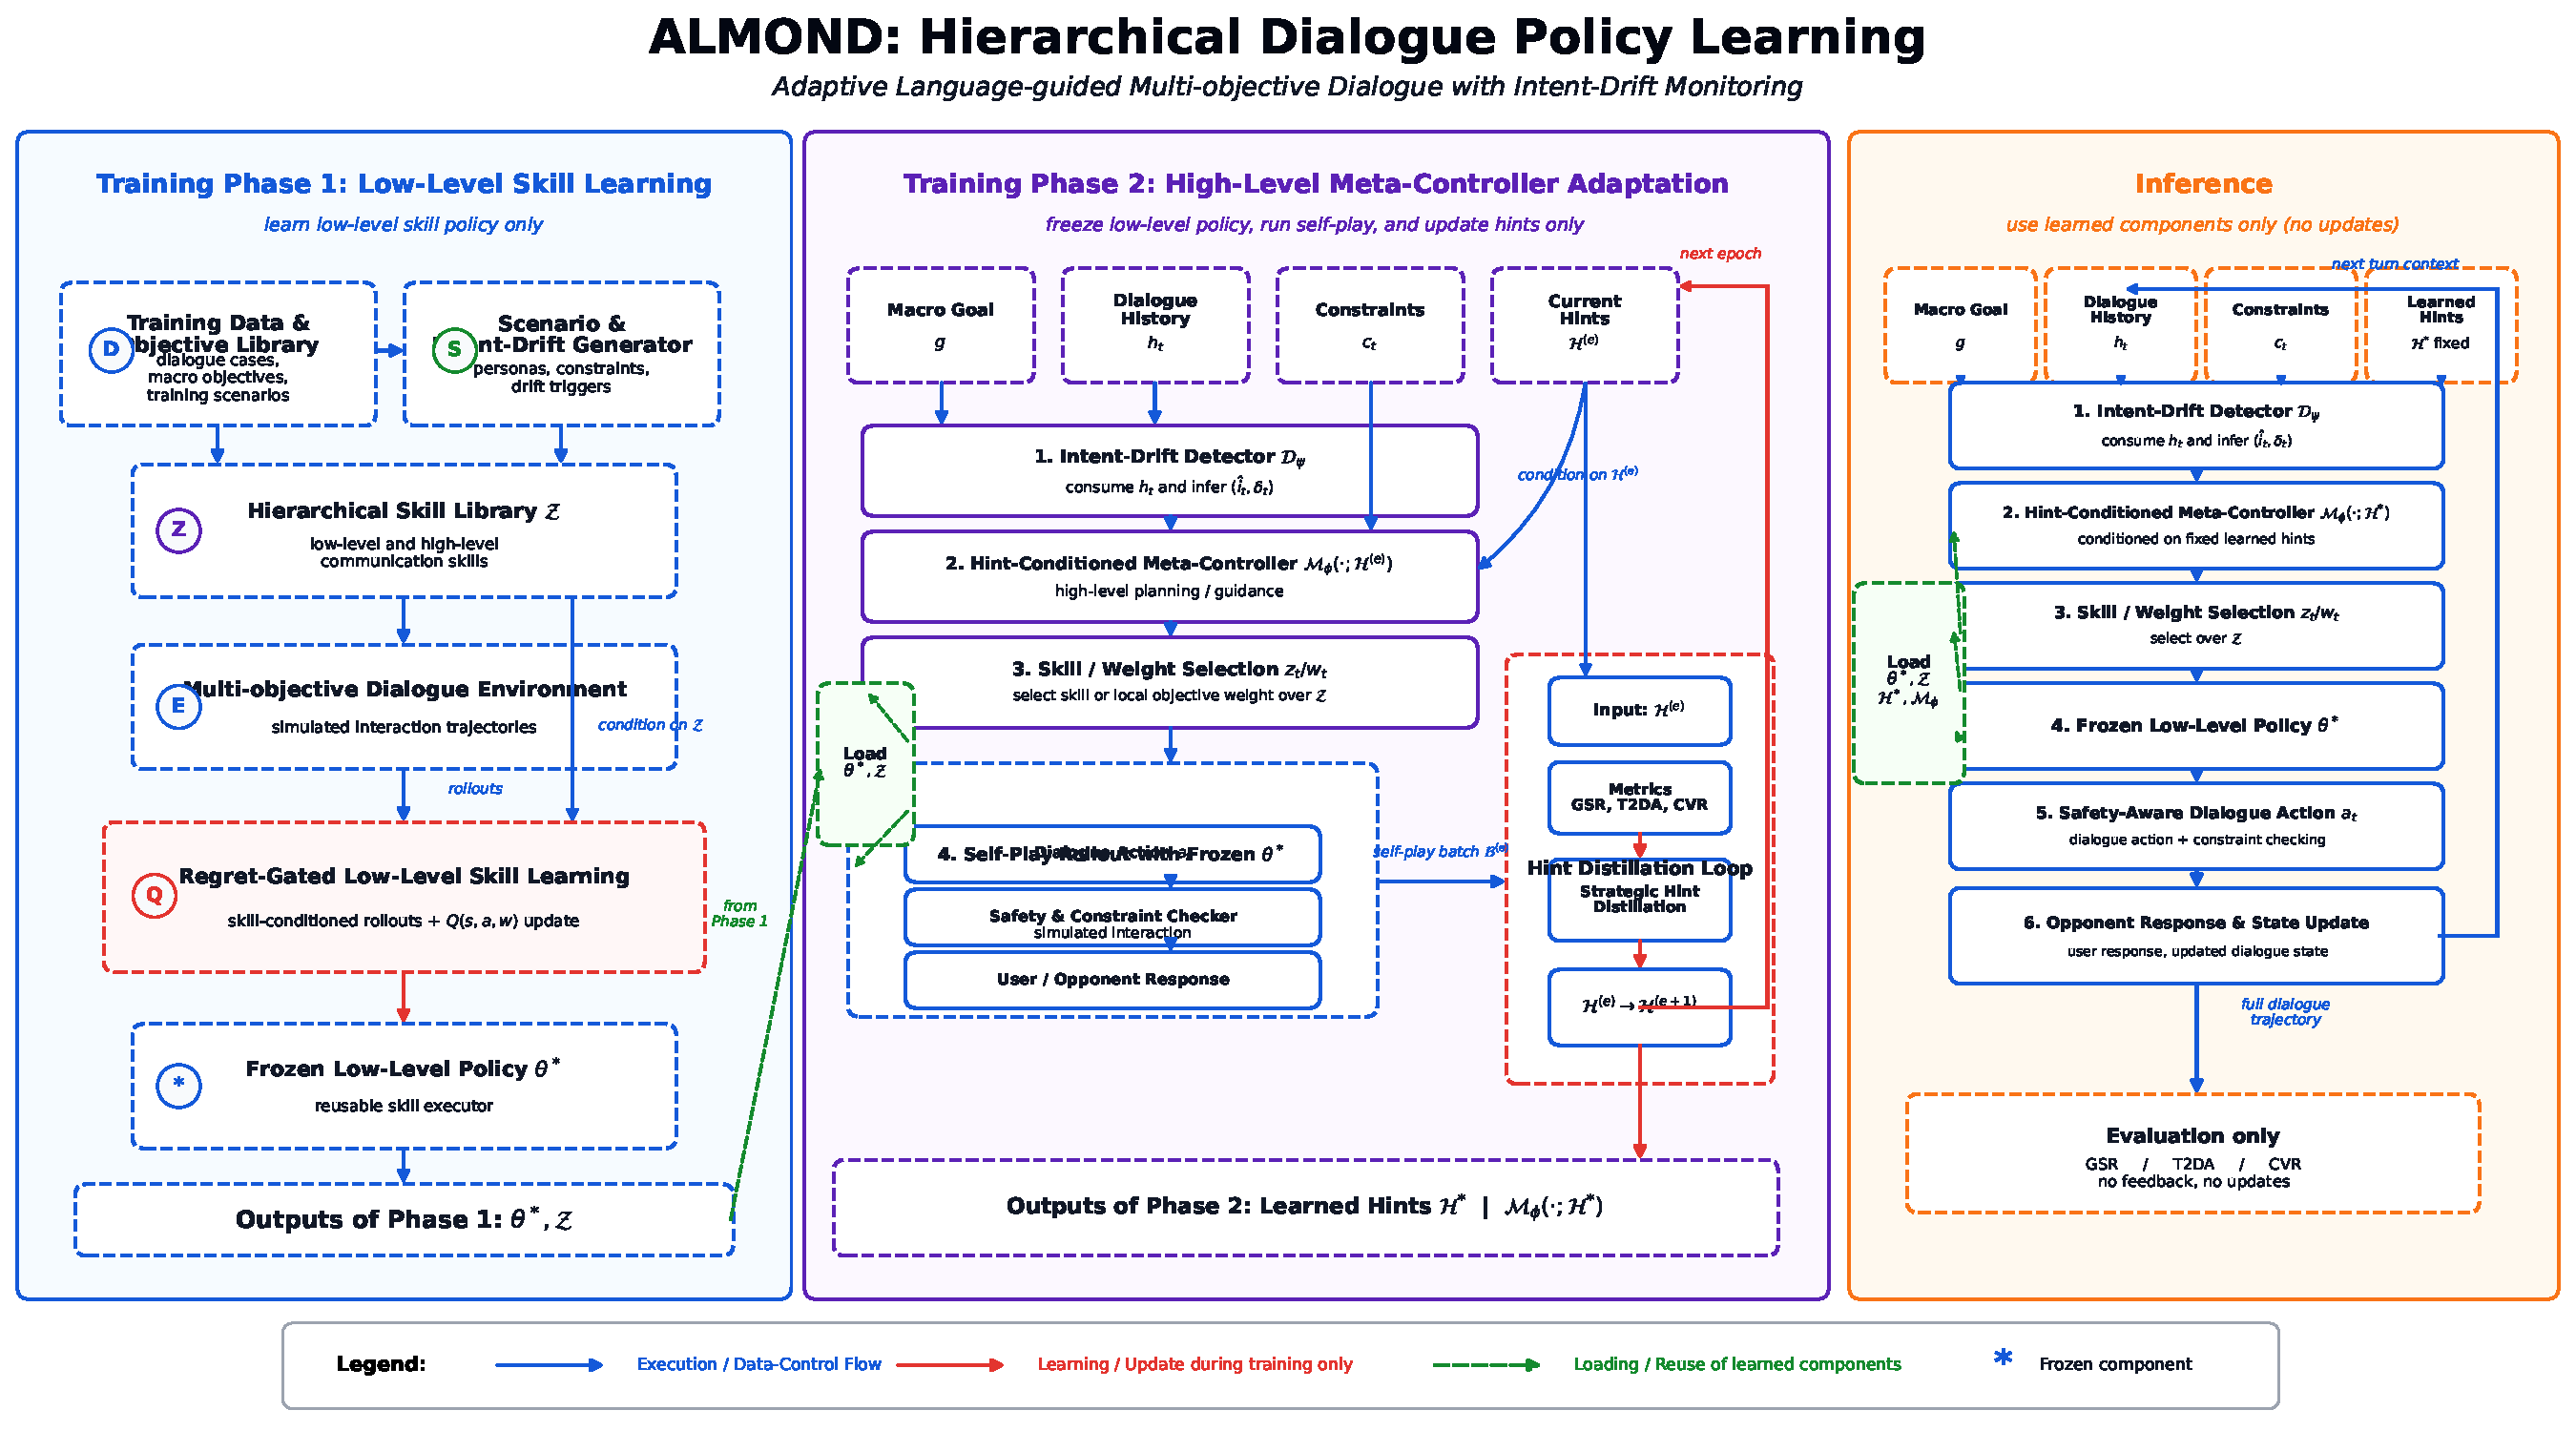
\includegraphics[width=\linewidth]{almond_correct_flow.pdf}
\caption{ALMOND decouples regret-based low-level skill learning from
intent-aware high-level skill selection.}
\label{fig:almond}
\end{figure}

\subsection{Phase 1: Regret-Based Universal Skill Learning}

The low-level policy operates in the same multi-objective action space as
preference-conditioned dialogue planners. In negotiation, a local skill is a
weight vector
$w \in \Delta^{2}$ over three primitive objectives:
\texttt{sl\_ratio}, \texttt{fairness}, and \texttt{deal\_rate}. These
dimensions correspond respectively to buyer price gain, relationship-preserving
fairness, and the probability of closing an agreement. Given a dialogue state
$s_t$, action $a_t$, and local skill $w$, the low-level network predicts a
vector action value $Q(s_t,a_t,w;\theta) \in \mathbb{R}^{3}$. The scalar reward
used for a particular skill is
\begin{equation}
    r_w(s_t,a_t) = w^{\top}r_t,
\end{equation}
where $r_t=[r^{gain}_t,r^{fair}_t,r^{deal}_t]$ is the environment reward
vector.

\textbf{Anchor skill curriculum.}
Training directly on arbitrary Dirichlet samples can make the policy unstable,
because early GPI targets may be produced by poorly learned preferences. ALMOND
first anchors the low-level policy at a small set of reliable skills:
\begin{equation}
    \mathcal{W}_{0} =
    \{e_1,e_2,e_3,u,m_{12},m_{23},m_{13}\}.
\end{equation}
Here $e_i$ are the three one-hot corner weights, $u=[1/3,1/3,1/3]$,
and $m_{ij}$ are the three edge midpoints.
Each Phase-1 episode samples one anchor and trains the policy with a self TD
target, without a GPI teacher:
\begin{equation}
    a_{\mathrm{self}} =
    \arg\max_{a'} w^{\top}Q(s_{t+1},a',w;\bar{\theta}),
\end{equation}
\begin{equation}
    y_{\mathrm{self}} =
    w^{\top}\left(r_t + \gamma(1-d_t)
    Q(s_{t+1},a_{\mathrm{self}},w;\bar{\theta})\right),
\end{equation}
\begin{equation}
    \mathcal{L}_{\mathrm{anchor}}(\theta)=
    \mathbb{E}\left[
    \left(y_{\mathrm{self}} -
    w^{\top}Q(s_t,a_t,w;\theta)\right)^2\right].
\end{equation}
This curriculum produces a set of stable basic skills that initialize the
converged-skill memory for later knowledge reuse.

\textbf{Regret-gated knowledge reuse.}
After anchor training, ALMOND expands from discrete skills to the continuous
simplex using a regret-aware variant of PADPP. We maintain a delayed snapshot
$Q(\cdot;\theta^-)$ of the current network and estimate the regret of a
candidate skill $w$ on a replay-buffer state batch:
\begin{equation}
    \mathrm{Reg}(w)=
    \mathbb{E}_{s,a}\left[
    \left|Q(s,a,w;\theta)-Q(s,a,w;\theta^-)\right|
    \right].
\end{equation}
Only skills whose regret is below a threshold $\epsilon$ are admitted to the
teacher set:
\begin{equation}
    \mathcal{W}_{\mathrm{conv}} =
    \{w \mid \mathrm{Reg}(w)<\epsilon\}.
\end{equation}
This gate prevents unstable or recently changed preferences from serving as
teachers. For a sampled training skill $w$, the GPI teacher action is selected
from converged skills only:
\begin{equation}
    a_{\mathrm{gpi}} =
    \arg\max_{a'}\max_{w_i \in \mathcal{W}_{\mathrm{conv}}}
    w^{\top}Q(s_{t+1},a',w_i;\bar{\theta}).
\end{equation}
The knowledge-reuse target evaluates the teacher action under the current
training skill:
\begin{equation}
    y_{\mathrm{know}} =
    r_t + \gamma(1-d_t)
    Q(s_{t+1},a_{\mathrm{gpi}},w;\bar{\theta}).
\end{equation}
The final low-level update mixes independent execution with regret-gated GPI:
\begin{equation}
    \mathcal{L}_{\mathrm{low}}(\theta)=
    (1-\alpha)\mathcal{L}_{\mathrm{self}}(\theta)
    + \alpha\mathcal{L}_{\mathrm{know}}(\theta).
\end{equation}
Here $\mathcal{L}_{\mathrm{self}}$ is the scalar DDQN-style TD loss under $w$,
and $\mathcal{L}_{\mathrm{know}}$ is the vector TD loss induced by
$a_{\mathrm{gpi}}$. During rollout, candidate skills can also be sampled in
proportion to $\mathrm{Reg}(w)^\beta$, which concentrates data collection on
under-mastered regions of the skill simplex.

\subsection{Phase 2: Intent-Aware High-Level Meta-Control}

Phase 1 learns how to execute a local skill, but it does not decide which skill
should be active for a natural-language macro-goal. In Phase 2, the low-level
checkpoint $\theta^{*}$ is frozen. A high-level controller produces a local
weight vector $w_t$ from the macro-goal $g$, the dialogue state $s_t$, hard
constraints $c$, the previous local skill, and the current estimate of seller
intent. The frozen low-level policy then selects the action:
\begin{equation}
    a_t =
    \arg\max_{a \in \mathcal{A}}
    w_t^{\top}Q(s_t,a,w_t;\theta^{*}).
\end{equation}

\textbf{Intent-drift detector.}
Because the true intent $i_t$ is hidden, ALMOND uses a detector to infer intent
from visible dialogue evidence:
\begin{equation}
    (\delta_t,\hat{i}_t)=
    \mathcal{D}_{\psi}(s_t,\hat{i}_{t-1},\mathcal{H}_{det}),
\end{equation}
where $\delta_t$ indicates whether the seller's intent has changed. The intent
catalog used in the implementation contains four states:
\textit{neutral}, \textit{firm}, \textit{final\_offer}, and
\textit{walkaway\_risk}. These states correspond to observable signals such as
ordinary bargaining, hardened price resistance, take-it-or-leave-it offers, and
frustrated threats to sell elsewhere.

\textbf{High-policy weight selection.}
The high policy regenerates $w_t$ at the beginning of the dialogue, when drift
is detected, or after a fixed macro horizon $K$. Let
\begin{equation}
    m_t=\mathbb{I}[t=0 \vee \delta_t=1 \vee t \bmod K=0].
\end{equation}
The local skill is updated as
\begin{equation}
    w_t =
    \begin{cases}
    \mathcal{M}_{\phi}(g,s_t,\hat{i}_t,c,w_{t-1},\mathcal{H}_{pol}),
    & m_t=1,\\
    w_{t-1}, & m_t=0.
    \end{cases}
\end{equation}
In the LLM controller path, $\mathcal{M}_{\phi}$ first emits an inspectable
natural-language allocation, e.g., percentages over price saving, fairness, and
deal closing, and the allocation is parsed into a normalized vector
$w_t=[w^{gain}_t,w^{fair}_t,w^{deal}_t]$. This explicit allocation makes the
macro decision auditable: under the same macro-goal, the controller may push
price gain while the seller is neutral but raise \texttt{deal\_rate} and
\texttt{fairness} when the seller becomes firm or signals walkaway risk.

\textbf{Safety masking.}
ALMOND treats hard buyer constraints as action-level constraints rather than
soft preferences. After the low-level policy proposes an action, a safety mask
checks whether the committed price violates the buyer ceiling. If it does, the
action is replaced by a ceiling-respecting counteroffer:
\begin{equation}
    \tilde{a}_t = \mathcal{M}_{safe}(a_t,c).
\end{equation}
This mask is deliberately outside the reward scalarization so that no temporary
skill allocation can justify overpaying.

\textbf{Hint distillation.}
The high-level controller is improved without retraining the low policy.
During self-play, each episode records the selected weights, detected intents,
drift events, blocked violations, and final constrained metrics. A distiller
turns these records into reusable natural-language hints:
\begin{equation}
    \mathcal{H}^{(e+1)} =
    \mathrm{Distill}_{\omega}
    \left(\mathcal{H}^{(e)},\mathcal{B}^{(e)},
    \mathrm{GSR}^{(e)},\mathrm{T2DA}^{(e)},\mathrm{CVR}^{(e)}\right),
\end{equation}
where $\mathcal{B}^{(e)}$ is the compact self-play digest at epoch $e$. In the
two-agent variant, ALMOND keeps separate hint memories for the detector and the
high policy. During training, gold simulator intent can supervise high-policy
refreshes while detector predictions are scored; at inference time, the detector
prediction drives the weight refresh. This design lets ALMOND adapt
macro-goals through explicit, reusable skill vectors while preserving the
general low-level competence learned in Phase 1.

\section{Experimental}

\subsection{Experimental Setup}

We design the experiments around three research questions.
\begin{itemize}
    \item \textbf{RQ1: Low-level skill learning.} Does the proposed
    Regret-Based Universal Skill Learning module improve low-level policy
    learning? We compare the Phase-1/Phase-2 low policy against PADPP under the
    PADPP negotiation protocol, with the uniform weight setting as the primary
    comparison and the three corner objectives as diagnostic settings.
    \item \textbf{RQ2: End-to-end macro-goal adaptation.} Does the complete
    two-phase ALMOND model improve performance on Macro Goals, where the input
    objective is expressed in natural language and seller intent may drift
    during the dialogue?
    \item \textbf{RQ3: Ablation study.} Which components are responsible for
    the gains? We evaluate variants that remove regret-gated GPI, dynamic
    high-level weight selection, intent detection, hint distillation, and the
    safety mask.
\end{itemize}

\textbf{Baselines.}
We compare ALMOND with four policy-planning baselines. \textit{PADPP}
\cite{dao-liao-2025-one} is the closest multi-objective baseline: it trains one
preference-conditioned planner and uses a fixed numerical preference vector
during an episode. In our macro-goal benchmark, the PADPP-static baseline uses
the scenario's initial mapped weight $\texttt{static\_w}$ throughout the
dialogue. \textit{PPDPP} \cite{deng2024plug} trains a plug-and-play policy
planner from human data and goal-oriented AI feedback, but does not explicitly
learn a dynamic local objective vector under intent drift. \textit{DPDP}
\cite{he2024planning} combines a fast policy model with deliberative MCTS
planning, providing a strong look-ahead planning baseline. \textit{TRIP}
\cite{zhang-etal-2024-strength} improves strategy planning for
non-collaborative dialogue through user-aware planning and diversified user
simulation. For RQ1, PADPP is the main baseline because both methods share the
same low-level multi-objective interface $Q(s,a,w)$.

\textbf{Datasets and scenario construction.}
We evaluate on two benchmark families: Bargain and Recommendation. Bargain is
derived from CraigslistBargain negotiation cases \cite{he-etal-2018-decoupling}.
For each case, we keep the item name, buyer and seller reference prices, item
descriptions, and source dialogue length. Recommendation is derived from the
English DuRecDial 2.0 corpus \cite{liu-etal-2021-durecdial}. Since DuRecDial is
a recommendation corpus and does not contain transaction prices, we convert its
movie, music, and point-of-interest cases into recommendation-derived
negotiation scenarios with deterministic synthetic price bands generated from a
fixed seed. This keeps the recommendation context reproducible while preserving
the same buyer-seller evaluation interface.

\begin{table*}[t]
\caption{Generated benchmark splits used for ALMOND evaluation.}
\label{tab:benchmark_splits}
\centering
\begin{tabular}{lccp{9.2cm}}
\hline
\textbf{Benchmark} & \textbf{Train} & \textbf{Test} & \textbf{Construction} \\
\hline
Bargain & 1000 & 250 &
CraigslistBargain cases with item context, buyer/seller prices, macro-goals,
buyer constraints, seller personas, deterministic drift modes, and expected
post-drift weight shifts. \\
Recommendation & 1000 & 250 &
DuRecDial-derived movie, music, and point-of-interest cases converted into the
same buyer-seller interface with deterministic synthetic prices and
recommendation-specific item context. \\
\hline
\end{tabular}
\end{table*}

The generated scenarios are balanced across four drift modes:
\textit{static\_no\_drift}, \textit{gradual\_firming},
\textit{abrupt\_final\_offer}, and \textit{frustrated\_walkaway}. Each scenario
contains a natural-language \texttt{macro\_goal}, a buyer intent identifier, an
initial static weight, a price ceiling, a target price, a turn limit, a seller
persona, a deterministic drift trigger, and an expected direction of weight
adaptation. Phase-1 experiments use the original negotiation policy-learning
protocol with the seven anchor weights in $\mathcal{W}_0$ and evaluate static
skills using the PADPP Table-2 style setting. Phase-2 experiments use the
generated macro-goal scenarios: training runs self-play and hint distillation on
the train splits, while final evaluation is conducted on the held-out test
splits.

\textbf{Evaluation metrics.}
For low-level policy learning (RQ1), we report the standard negotiation metrics
used by PADPP: Success Rate (SR), average dialogue turns, $r_{gain}$,
$r_{fair}$, and $r_{deal}$. Following the implementation, $r_{gain}$,
$r_{fair}$, and $r_{deal}$ are averaged over the agent decision turns in an
episode.

For macro-goal adaptation (RQ2 and RQ3), we report four constrained adaptation
metrics. \textit{LLM-SR} is the judge-based rate at which the dialogue reaches
the intended outcome, with human audit samples exported for verification.
\textit{Goal Success Rate} (GSR) is stricter:
\begin{equation}
    \mathrm{GSR} =
    \mathbb{I}[\mathrm{deal}=1
    \wedge p_{\mathrm{deal}}\le p_{\mathrm{ceiling}}
    \wedge T_{\mathrm{dialogue}}\le T_{\mathrm{limit}}].
\end{equation}
\textit{Turn-to-Drift Adaptation Delay} (T2DA) measures how quickly the
controller changes its local skill after the seller intent drifts:
\begin{equation}
    \mathrm{T2DA}=t_{\mathrm{adapt}}-t_{\mathrm{drift}},
\end{equation}
where $t_{\mathrm{adapt}}$ is the first turn after drift where
$\lVert w_t-w_{\mathrm{pre}}\rVert_1 \ge 0.25$ and the shift follows the
expected direction. \textit{Constraint Violation Rate} (CVR) measures the
fraction of turns that attempt or execute an over-ceiling buyer action; we
report blocked and actual violations separately. Higher is better for SR,
$r_{gain}$, $r_{fair}$, $r_{deal}$, LLM-SR, and GSR; lower is better for
average turns, T2DA, and CVR.

\subsection{Experimental Results}

We organize the results according to the three research questions. The first
block reports whether regret-based low-level training improves the static
uniform and anchor-weight skills over PADPP. The second block evaluates the full
two-phase ALMOND system on Bargain and Recommendation macro-goal scenarios. The
third block reports ablations over regret gating, dynamic high-level control,
intent detection, hint distillation, and safety masking.

\iffalse
\section{Proposed Method}

To effectively solve the formulated NL-POMDP and achieve a high success rate in the face of latent user intent drift, ALMOND decouples the complex, language-guided decision-making process into a hierarchical two-phase architecture:

\begin{itemize}
    \item \textbf{Phase 1: Regret-Based Universal Skill Learning (Low-Level Policy).} In this phase, the agent trains a universal low-level policy to master a continuous space of communication skills for short-term, micro-numeric objectives. To achieve zero-shot execution of arbitrary skill vectors without retraining, this acquisition is driven by a novel regret-based mechanism that dynamically prioritizes unmastered skills based on their regret signals. This proficiency-aware approach fosters robust inter-skill knowledge sharing, allowing easily mastered skills to bootstrap the learning of more complex behaviors across the entire skill space.
    
    \item \textbf{Phase 2: Intent Tracking and Meta-Control (High-Level Policy).} Leveraging the foundation of acquired universal skills, this phase employs an LLM as a strategic meta-controller. Its mission is to satisfy the overarching natural language macro-objective by continuously monitoring the dialogue context for latent user intent drift, adaptively selecting the optimal short-term skill for the low-level policy to execute. To optimize this decision-making process, the meta-controller utilizes an experience collection mechanism during training, distilling interaction outcomes into a repository of strategic hints to guide robust, on-the-fly skill selection during inference.
\end{itemize}

In the following subsections, we detail the operational mechanics and mathematical formulations of each phase.

\subsection{Phase 1: Regret-Aware Adaptive Skill Learning}

In the ALMOND framework, a communication skill is defined as a specific behavioral strategy conditioned on a micro-objective. Sharing the environment settings with \cite{dao-liao-2025-one}, these short-term objectives, denoted as $w$, are formulated as dense numerical vectors on a simplex. Each dimension within $w$ corresponds to a specific primitive objective defined by domain experts---such as price utility, dialogue fairness, or agreement probability---where the scalar value dictates its relative priority during the negotiation. 

The primary goal of this phase is to train a universal low-level Q-network, $Q(s, a, w; \theta)$, capable of maximizing the expected cumulative return by dynamically trading off primitive objectives exactly as prioritized by any given $w$. To achieve this, executing an action yields a multi-dimensional reward vector $r_{micro}$, representing the absolute performance across all primitive criteria. The scalarized step reward is computed via the inner product:
\begin{equation}
    r_w = w^{\top} r_{micro}
\end{equation}

To efficiently master the continuous skill space without gradient instability, the training process is decoupled into an anchor initialization curriculum followed by a regret-gated knowledge reuse mechanism.

\textbf{Anchor Curriculum Initialization.} Learning a continuous preference space from scratch is highly unstable. Thus, we pre-train the Q-network on a discrete set of anchor preferences that uniformly span the objective simplex (e.g., corners and midpoints). During this phase, the network updates strictly via self-learning Temporal Difference (TD) loss without external teacher forcing. This firmly anchors the neural representations, providing a robust initialization for the subsequent continuous generalization. These anchor preferences are inherently stable and form the initial set of converged policies.

\textbf{Regret Tracking and Active Sampling.} Transitioning to the continuous simplex, the agent must actively explore unstable regions. We define the \textit{regret} of a preference $w$ as the temporal fluctuation of its Q-values. By maintaining a delayed snapshot network parameterized by $\theta_{old}$, the regret is quantified across a sampled state batch:
\begin{equation}
    \mathrm{Reg}(w) = \mathbb{E}_{s,a} \left[ \lvert Q(s, a, w; \theta) - Q(s, a, w; \theta_{old}) \rvert \right]
\end{equation}
During environment interaction, we sample random Dirichlet preferences and intentionally select the one exhibiting the highest regret for trajectory rollout. This active sampling forces the agent to collect exploratory data in regions where its policy is least stable.

\textbf{Regret-Gated Generalized Policy Improvement (GPI).} A well-known limitation of standard GPI in multi-objective RL is the injection of noisy gradients when utilizing non-converged preferences as teachers. To mitigate this "moving target" problem, we introduce a Regret-Gated buffer, $\mathcal{W}_{converged}$, which strictly admits preferences whose regret falls below a threshold $\epsilon$. For any training preference $w$, the target action is guided solely by this elite set of stabilized teachers:
\begin{equation}
    \pi_{teacher}(s') = \arg\max_{a} \max_{w_i \in \mathcal{W}_{converged}} w^{\top} Q(s', a, w_i; \theta_{target})
\end{equation}

\textbf{Optimization Objective.} The final parameter update per minibatch balances independent skill execution and teacher-guided knowledge sharing. The total loss is a weighted sum:
\begin{equation}
    \mathcal{L}(\theta) = (1 - \alpha)\mathcal{L}_{self}(\theta) + \alpha\mathcal{L}_{know}(\theta)
\end{equation}
where $\mathcal{L}_{self}(\theta)$ is the standard Deep Q-Network loss derived from the agent's own greedy action, and $\mathcal{L}_{know}(\theta)$ minimizes the temporal difference error using the target value proposed by $\pi_{teacher}$. This regret-aware pipeline ensures stable, zero-shot generalization across arbitrary micro-objectives.

\subsection{Phase 2: High-Level Meta-Controller and Hint Distillation}

Phase 1 solves only half of the problem: it learns how to execute a skill once a
numeric micro-objective is given. The remaining gap is the one left open by
preference-conditioned planners such as PADPP: real users specify goals in
language, and the correct short-term preference is not static when the
counterparty's intent drifts. Phase 2 addresses this gap by learning a
high-level meta-controller that translates a stable macro-goal $g$ into a
time-varying sequence of local skill vectors $\{w_t\}$.

At turn $t$, the meta-controller observes the dialogue state $s_t$, the
previously active skill $w_{t^-}$, hard constraints $c$, and a distilled hint
memory $\mathcal{H}$. It selects a local objective vector $w_t$ over the
primitive objectives mastered in Phase 1. The frozen low-level policy then
executes the corresponding skill:
\begin{equation}
    a_t = \arg\max_{a \in \mathcal{A}} w_t^{\top} Q(s_t, a, w_t; \theta^*),
\end{equation}
where $\theta^*$ denotes the Phase-1 checkpoint. This separation is crucial:
the low-level policy provides reusable competence, while the high-level policy
provides situational judgment.

\textbf{Intent-Aware Meta-Control.}
The meta-controller must decide not only what the macro-goal means, but also
when its local interpretation should change. ALMOND therefore introduces an
intent-drift detector that estimates the current latent intent from textual
evidence:
\begin{equation}
    (\delta_t, \hat{i}_t)=
    \mathcal{D}_{\psi}(s_t,\hat{i}_{t-1},\mathcal{H}_{det}),
\end{equation}
where $\delta_t$ indicates whether a drift is detected. This detector closes the
observability gap in the NL-POMDP formulation: the true intent $i_t$ is hidden,
but its traces appear in rejections, final-offer language, or walkaway signals.
The controller refreshes the local skill only at macro-decision points: the
first turn, every $K$ turns, or when $\delta_t=1$. Let
$m_t=\mathbb{I}[t=1 \vee (t \bmod K=0) \vee \delta_t=1]$. The high-level update
is:
\begin{equation}
    w_t = m_t\mathcal{M}_{\phi}(g,s_t,\hat{i}_t,c,w_{t^-},\mathcal{H})
    +(1-m_t)w_{t-1}.
\end{equation}
In practice, $\mathcal{M}_{\phi}$ is an LLM controller that first states an
inspectable natural-language allocation, e.g., assigning percentages to price
gain, fairness, and deal probability, and then normalizes that allocation into
$w_t$. This makes the control signal both executable and auditable: the same
macro-goal can legitimately map to price-seeking behavior while the seller is
flexible, but to deal-seeking or fairness-preserving behavior after final-offer
or walkaway cues. A safety mask is applied after low-level action selection so
that hard constraints such as the buyer's budget ceiling remain enforceable
even when the controller trades off soft objectives.

\textbf{Hint Distillation.}
The final challenge is that the meta-controller needs strategic feedback, not
just fluent reasoning. ALMOND therefore improves the controller through
self-play and hint distillation rather than low-level retraining. During
training, the frozen policy interacts with intent-drifting simulators while the
meta-controller selects $\{w_t\}$. Each episode is summarized by selected
weights, inferred intents, safety-mask events, and constrained adaptation
metrics: GSR for goal success under budget and turn constraints, T2DA for
adaptation delay after drift, and CVR for constraint violations. At epoch $e$,
an LLM distiller rewrites the hint memory from the current playbook and episode
digest:
\begin{equation}
    \mathcal{H}^{(e+1)} =
    \mathrm{Distill}_{\omega}
    (\mathcal{H}^{(e)},\mathcal{B}^{(e)},
    \mathrm{GSR}^{(e)},\mathrm{T2DA}^{(e)},\mathrm{CVR}^{(e)}),
\end{equation}
where $\mathcal{B}^{(e)}$ is a compact self-play summary. The resulting hints
are general, transferable rules for when to shift $w_t$, such as reacting
quickly to final-offer cues while preserving the price ceiling. In the
two-agent variant, ALMOND maintains separate hint memories for intent detection
and high-policy weight selection. Thus Phase 2 directly addresses the research
gap: it converts natural-language goals and drift evidence into adaptive
short-term skills, while preserving the reusable low-level competence learned
in Phase 1.


Before you begin to format your paper, first write and save the content as a 
separate text file. Complete all content and organizational editing before 
formatting. Please note sections \ref{AA}--\ref{SCM} below for more information on 
proofreading, spelling and grammar.

Keep your text and graphic files separate until after the text has been 
formatted and styled. Do not number text heads---{\LaTeX} will do that 
for you.

\subsection{Abbreviations and Acronyms}\label{AA}
Define abbreviations and acronyms the first time they are used in the text, 
even after they have been defined in the abstract. Abbreviations such as 
IEEE, SI, MKS, CGS, ac, dc, and rms do not have to be defined. Do not use 
abbreviations in the title or heads unless they are unavoidable.

\subsection{Units}
\begin{itemize}
\item Use either SI (MKS) or CGS as primary units. (SI units are encouraged.) English units may be used as secondary units (in parentheses). An exception would be the use of English units as identifiers in trade, such as ``3.5-inch disk drive''.
\item Avoid combining SI and CGS units, such as current in amperes and magnetic field in oersteds. This often leads to confusion because equations do not balance dimensionally. If you must use mixed units, clearly state the units for each quantity that you use in an equation.
\item Do not mix complete spellings and abbreviations of units: ``Wb/m\textsuperscript{2}'' or ``webers per square meter'', not ``webers/m\textsuperscript{2}''. Spell out units when they appear in text: ``. . . a few henries'', not ``. . . a few H''.
\item Use a zero before decimal points: ``0.25'', not ``.25''. Use ``cm\textsuperscript{3}'', not ``cc''.)
\end{itemize}

\subsection{Equations}
Number equations consecutively. To make your 
equations more compact, you may use the solidus (~/~), the exp function, or 
appropriate exponents. Italicize Roman symbols for quantities and variables, 
but not Greek symbols. Use a long dash rather than a hyphen for a minus 
sign. Punctuate equations with commas or periods when they are part of a 
sentence, as in:
\begin{equation}
a+b=\gamma\label{eq}
\end{equation}

Be sure that the 
symbols in your equation have been defined before or immediately following 
the equation. Use ``\eqref{eq}'', not ``Eq.~\eqref{eq}'' or ``equation \eqref{eq}'', except at 
the beginning of a sentence: ``Equation \eqref{eq} is . . .''

\subsection{\LaTeX-Specific Advice}

Please use ``soft'' (e.g., \verb|\eqref{Eq}|) cross references instead
of ``hard'' references (e.g., \verb|(1)|). That will make it possible
to combine sections, add equations, or change the order of figures or
citations without having to go through the file line by line.

Please don't use the \verb|{eqnarray}| equation environment. Use
\verb|{align}| or \verb|{IEEEeqnarray}| instead. The \verb|{eqnarray}|
environment leaves unsightly spaces around relation symbols.

Please note that the \verb|{subequations}| environment in {\LaTeX}
will increment the main equation counter even when there are no
equation numbers displayed. If you forget that, you might write an
article in which the equation numbers skip from (17) to (20), causing
the copy editors to wonder if you've discovered a new method of
counting.

{\BibTeX} does not work by magic. It doesn't get the bibliographic
data from thin air but from .bib files. If you use {\BibTeX} to produce a
bibliography you must send the .bib files. 

{\LaTeX} can't read your mind. If you assign the same label to a
subsubsection and a table, you might find that Table I has been cross
referenced as Table IV-B3. 

{\LaTeX} does not have precognitive abilities. If you put a
\verb|\label| command before the command that updates the counter it's
supposed to be using, the label will pick up the last counter to be
cross referenced instead. In particular, a \verb|\label| command
should not go before the caption of a figure or a table.

Do not use \verb|\nonumber| inside the \verb|{array}| environment. It
will not stop equation numbers inside \verb|{array}| (there won't be
any anyway) and it might stop a wanted equation number in the
surrounding equation.

\subsection{Some Common Mistakes}\label{SCM}
\begin{itemize}
\item The word ``data'' is plural, not singular.
\item The subscript for the permeability of vacuum $\mu_{0}$, and other common scientific constants, is zero with subscript formatting, not a lowercase letter ``o''.
\item In American English, commas, semicolons, periods, question and exclamation marks are located within quotation marks only when a complete thought or name is cited, such as a title or full quotation. When quotation marks are used, instead of a bold or italic typeface, to highlight a word or phrase, punctuation should appear outside of the quotation marks. A parenthetical phrase or statement at the end of a sentence is punctuated outside of the closing parenthesis (like this). (A parenthetical sentence is punctuated within the parentheses.)
\item A graph within a graph is an ``inset'', not an ``insert''. The word alternatively is preferred to the word ``alternately'' (unless you really mean something that alternates).
\item Do not use the word ``essentially'' to mean ``approximately'' or ``effectively''.
\item In your paper title, if the words ``that uses'' can accurately replace the word ``using'', capitalize the ``u''; if not, keep using lower-cased.
\item Be aware of the different meanings of the homophones ``affect'' and ``effect'', ``complement'' and ``compliment'', ``discreet'' and ``discrete'', ``principal'' and ``principle''.
\item Do not confuse ``imply'' and ``infer''.
\item The prefix ``non'' is not a word; it should be joined to the word it modifies, usually without a hyphen.
\item There is no period after the ``et'' in the Latin abbreviation ``et al.''.
\item The abbreviation ``i.e.'' means ``that is'', and the abbreviation ``e.g.'' means ``for example''.
\end{itemize}
An excellent style manual for science writers is \cite{b7}.

\subsection{Authors and Affiliations}
\textbf{The class file is designed for, but not limited to, six authors.} A 
minimum of one author is required for all conference articles. Author names 
should be listed starting from left to right and then moving down to the 
next line. This is the author sequence that will be used in future citations 
and by indexing services. Names should not be listed in columns nor group by 
affiliation. Please keep your affiliations as succinct as possible (for 
example, do not differentiate among departments of the same organization).

\subsection{Identify the Headings}
Headings, or heads, are organizational devices that guide the reader through 
your paper. There are two types: component heads and text heads.

Component heads identify the different components of your paper and are not 
topically subordinate to each other. Examples include Acknowledgments and 
References and, for these, the correct style to use is ``Heading 5''. Use 
``figure caption'' for your Figure captions, and ``table head'' for your 
table title. Run-in heads, such as ``Abstract'', will require you to apply a 
style (in this case, italic) in addition to the style provided by the drop 
down menu to differentiate the head from the text.

Text heads organize the topics on a relational, hierarchical basis. For 
example, the paper title is the primary text head because all subsequent 
material relates and elaborates on this one topic. If there are two or more 
sub-topics, the next level head (uppercase Roman numerals) should be used 
and, conversely, if there are not at least two sub-topics, then no subheads 
should be introduced.

\subsection{Figures and Tables}
\paragraph{Positioning Figures and Tables} Place figures and tables at the top and 
bottom of columns. Avoid placing them in the middle of columns. Large 
figures and tables may span across both columns. Figure captions should be 
below the figures; table heads should appear above the tables. Insert 
figures and tables after they are cited in the text. Use the abbreviation 
``Fig.~\ref{fig}'', even at the beginning of a sentence.

\begin{table}[htbp]
\caption{Table Type Styles}
\begin{center}
\begin{tabular}{|c|c|c|c|}
\hline
\textbf{Table}&\multicolumn{3}{|c|}{\textbf{Table Column Head}} \\
\cline{2-4} 
\textbf{Head} & \textbf{\textit{Table column subhead}}& \textbf{\textit{Subhead}}& \textbf{\textit{Subhead}} \\
\hline
copy& More table copy$^{\mathrm{a}}$& &  \\
\hline
\multicolumn{4}{l}{$^{\mathrm{a}}$Sample of a Table footnote.}
\end{tabular}
\label{tab1}
\end{center}
\end{table}

\begin{figure}[htbp]
\centerline{\includegraphics{fig1.png}}
\caption{Example of a figure caption.}
\label{fig}
\end{figure}

Figure Labels: Use 8 point Times New Roman for Figure labels. Use words 
rather than symbols or abbreviations when writing Figure axis labels to 
avoid confusing the reader. As an example, write the quantity 
``Magnetization'', or ``Magnetization, M'', not just ``M''. If including 
units in the label, present them within parentheses. Do not label axes only 
with units. In the example, write ``Magnetization (A/m)'' or ``Magnetization 
\{A[m(1)]\}'', not just ``A/m''. Do not label axes with a ratio of 
quantities and units. For example, write ``Temperature (K)'', not 
``Temperature/K''.

\section*{Acknowledgment}

The preferred spelling of the word ``acknowledgment'' in America is without 
an ``e'' after the ``g''. Avoid the stilted expression ``one of us (R. B. 
G.) thanks $\ldots$''. Instead, try ``R. B. G. thanks$\ldots$''. Put sponsor 
acknowledgments in the unnumbered footnote on the first page.


\fi

\bibliographystyle{IEEEtran}
\bibliography{reference}
\end{document}
